\chapter{State of the art und Grundlagen}
Die Verkehrsstrategie des Senats sieht vor, dass das Radfahren bis zum Jahr 2025 20 Prozent des Gesamtverkehrs ausmachen soll. \cite{Mopo}
"Wir brauchen eine intelligente Konstruktion, die alle Verkehrsarten verbindet", sagte Stadtentwicklungssenator Michael Müller (SPD).\\
Für Autos gibt es bereits funktionierende \gls{App}s wie EnLighten und SignalGuru, aber auch Projekte mit eingebauten Systemen im Autocomputer, welche anstreben den Verkehr elektronisch optimieren.\\\\
Mehrere Möglichkeiten
Verkehrszentrale -- trotzdem gibt es manuell geschaltete Ampeln\\
% ### Auto ###
\section{State of the art}
\gls{V2X}- Kommunikation, GLOSA
Für den Einsatz in Kraftfahrzeugen gibt es bereits Projekte zu Ampelassistenten in Bordcomputern, Navigationssystemen, oder aber auch als App die rote Ampeln erkennen und die optimale Fahrtgeschwindigkeit ermitteln.
\subsection{Projekt Wolfsburger Welle}
Die \gls{VW}-Forschung initiierte in den 80er Jahren mit dem Projekt "'Wolfsburger Welle"' die ersten Untersuchungen zur "'Grünen Welle"' Informationen im Fahrzeug; mit der Idee, beim Annähern an eine Ampel die optimale Geschwindigkeit im Fahrzeug zu geben.\footnote{\cite{Welle}} "Dazu sendet die Ampelanlage ihren aktuellen Phasenzustand und eine Prognose für den nächsten Zustandwechsel an alle Fahrzeuge, die sich annähern. Der Fahrzeugcomputer setzt dann die aktuelle Fahrzeuggeschwindigkeit mit dem Abstand zur Ampel und der aktuellen Ampelphase in Bezug. Daraus wird errechnet, ob das Fahrzeug im Moment mit der grünen Welle ’mitschwimmt’ oder ob die Geschwindigkeit außerhalb des optimalen Bereichs liegt" \cite{MenschMaschine}.
\subsection{Projekt Travolution}
Im Sommer 2008 wurde das Projekt TRAVOLUTION\footnote{\cite{Travolution}} (TRAffic \& eVOLUTION), von dem Amt für Verkehrsmanagement und Geoinformation der Stadt Ingolstadt, Audi AG\footnote{Automobilhersteller, dem Volkswagen-Konzern zugehörig}, GEVAS Software und dem Lehrstuhl für Verkehrstechnik an der Technischen Universität München abgeschlossen. Es besteht aus den Teilprojekten \textsc{verkehrsadaptive Netzsteuerung mit Genetischen Algorithmen} und \textsc{Der informierte Fahrer}. Im Netzsteuerungsprojekt wurden 46 Lichtsignalanlagen in Ingolstadt mit der Netzsteuerungssoftware BALANCE ausgestattet, wodurch sie intelligent auf den Verkehr reagieren und die Schaltung an den Verkehr anpassen. 
\begin{figure}[H]  
    \centering  
    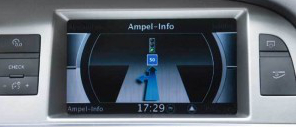
\includegraphics[scale=0.65]{audi-travolution}
    \label{fig:travolution}
    \caption[Projekt Travolution]{\gls{V2I}-Kommunikation: Der Bordcomputer zeigt die optimale Geschwindigkeit an, sodass die nächste Kreuzung ohne Halt überquert werden kann. Quelle: \cite{AudiTravolution}}
\end{figure}
Ziel des zweiten Teilprojektes ist es, die Autofahrer über die Ampelphasen zu informieren. Die \gls{V2I}-Kommunikation mittels WLAN umsetzend, senden mit Kommunikationsmodulen ausgestattete Ampeln die Grünphasen an den Bordcomputer der Autos, welcher widerum die Geschwindigkeit für ein reibungsloses Passieren errechnet.
\subsection{Projekt Testfeld Telematik}
Toyotas System erfordert eine spezielle Infrastruktur an Kreuzungen, die Installation von Infrarot-Sendern, die mit dem Toyota-Navigationssystem kommunizieren. An roter Ampel werden die Fahrer über die verbleibende Wartezeit informiert.\footnote{\cite{Toyota}}\\
Andere Autohersteller wie BMW, Volvo und Volkswagen kooperieren in diesem Forschungsprojekt, mit dem Forschungziel die Sicherheit an Kreuzungen zu verbessern. Im Auto installierte Sensoren kommunizieren mit Kameras und Scanner in der Ampel. \\
Allerdings funktioniert das System nur mit dem ambitionierten Ziel, wenn alle Autohersteller zusammenarbeiten und sich auf den gleichen Standard einigen.\footnote{\cite{Siemens}}
% ### Apps ### 
\subsection{EnLighten}
Die \gls{App} EnLighten erkennt rote Ampeln und visualisiert die Dauer dieser Phase.  
EnLighten nutzt \gls{GPS} zur Lokalisierung des Autos und verwendet die \gls{V2R}-Kommunikation zu Ampelphasenprognose.
\begin{figure}[H]
    \centering
    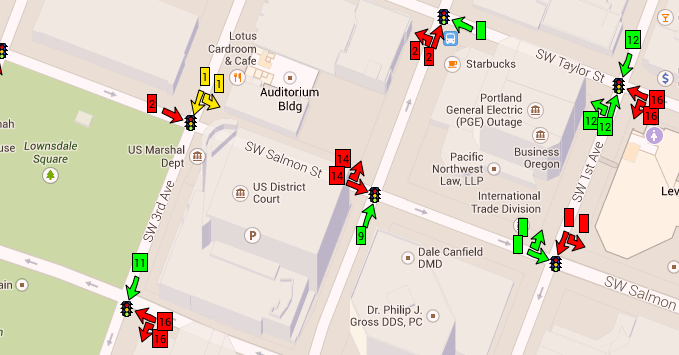
\includegraphics[scale=0.5]{EnLighten}
    \label{fig:Ampelsignalstatus}
    \caption[Echtzeit Ampelsignalstatus]{Schnappschuss der Echtzeit Ampelsignalstatusprognose in Portland. Quelle: \cite{EnLighten}}
\end{figure}
Hierbei verbindet sich die App über \gls{DSRC} mit den Lichtsignalanlagen und beachtet dabei Komponenten wie die Höchstgeschwindigkeit, Fahrtrichtung und Tageszeit.
Die Installation der \gls{DSRC}-Hardware an den Komponenten ist sehr aufändig und teuer, weswegen EnLighten erst in einigen amerikanischen Städten funktionstüchtig ist.
\subsection{Signal Guru}
Signal Guru wurde von den Wissenschaftlern des \gls{MIT} und der Universität von Princeton entwickelt. Die App errechnet über die Smartphones vieler Nutzer - welche miteinander kommunizieren -  die Wahrscheinlichkeit, wann eine Ampel grün wird und wie das eigene Fahrverhalten entsprechend anzupassen ist. Wie in Abbildung \ref{fig:AppSignalGuru} ist zu sehen ist, muss die eingebaute Kamera durch die Windschutzscheibe die Ampel registrieren. Bei Testläufen im Straßenverkehr vielen die Ergebnise bei statisch geschalteten Ampeln deutlich besser aus als bei angepassten Ampelschaltungen \footnote{Vgl. \cite{SignalGuru}} 
\begin{figure}[H]
    \centering
    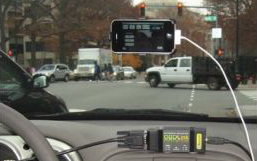
\includegraphics[scale=0.9]{SignalGuru}
    \caption[Signal Guru]{Signal Guru App muss in der Lage sein die Ampel zu 'sehen'.  Quelle: \cite{SignalGuruPaper}}
    \label{fig:AppSignalGuru}
\end{figure}
\textit{Ob das auch in Deutschland funktioniert ist schwer zu sagen, da die Ampeln hierzulande so gesetzt sind, dass das Smartphone in der Pole-Position die Ampel evtl. nicht erfassen kann. Dies gilt es in der Entwicklungsarbeit zu testen und gegebenenfalls auszuarbeiten.}
\subsection{Ampelmeter}
Ampelmeter ist eine Anwendung, die eine Geschwindigkeitsempfehlung angibt, bei der man die in Fahrtrichtung nächste Ampel bei grün erreichen. Der zweite Anwendungsfall ist die Restrot- bzw. Restgrünanzeige.\\
Da der timingbezogene Teil der Datenbank zum Startzeitpunkt noch leer ist, bedarf es etwas Mitarbeit der NutzerInnen.
\subsection{Analyseergebnis}
Diese Beispiele zeigen deutlich, dass die Nachfrage nach Ampelassistenten -- mobil oder statisch -- steigt und auf dem Markt Anklang findet. Der Verkehr ist flüssiger, die Teilnehmer entspannter, die Luft sauberer. AutofahrerInnen sind schon lange nicht mehr allein auf der Straße und so gilt es, dieses erfolgreiche Konzept für alle VerkehrteilnehmerInnen zu erweitern.
% ### Technische Grundlagen ###
\section{Technische Grundlagen}
\subsection{Arduino / Android-App}
\subsubsection{Mobile Sensing}
\textit{Der Beschleunigungssensor ist ein Hardwaresensor, der dazu benutzt wird, Position, Bewegung, Neigung, Erschütterung, Vibration und natürlich Beschleunigung des Gerätes zu messen.Es gibt bis zu 3-Achsen Beschleunigungssensoren, die meistens zum Erkennen der Ausrichtung des Smartphones genutzt werden und somit das Display beim Anschauen von Bildern, Webbrowsern oder Musikplayern in die passende Richtung vom Portrait-Modus (senkrecht) zum Landscape-Modus (waagrecht) zu drehen. In Kombination mit \gls{GPS} kann das Smartphone dank ihm sogar erkennen, welche Art Transportmittel (Fahrrad, Bus, U-Bahn) der Nutzer gerade benutzt und bestimmte Muster wie z.B. Rennen, Gehen oder Stehen unterscheiden.\\
GPS oder Global Positioning System erlaubt dem Smartphone sich selber zu lokalisieren und den exakten Standpunkt auf der Erde zu bestimmen. Es hilft locationbased\footnote{ortsgebunden} Apps wie z.B Navigation, lokale Suche nach Shops, Restaurants etc. oder soziale Netzwerke wie Facebook oder Foursquare nötige Informationen zu ermitteln. Der Kompass erweitert die Möglichkeiten der Lokalisationsermittlung eines Smartphones. Er bestimmt den Winkel des Geräts relativ zum Nordpol der Erde. Der Kompass besitzt einen Magnet, der mit dem magnetischen Feld der Erde interagiert und sich entsprechend zu einem der Pole ausrichtet. Zusammen mit dem Gyroskop Sensor verbessern GPS und Kompass die Präzision von locationbased Applikationen.Der Gyroskop Sensor bestimmt die Rotations- und Drehgeschwindigkeit des Smartphones auf seinen drei Achsen gegenüber dem Weltkoordinatensystem.}
\subsection{Backend mit nodejs / socket.io und MongoDB}
\subsection{Open-Street-Map}
